% \documentclass[dvipdfmx]{beamer}

% \usepackage{beamerthemesplit}
% \usepackage[]{graphicx}
\graphicspath{%
{./slide08-img/}%
{./text08-img/}%
}

% \usepackage{listings}
% \usepackage{hyperref}
% \usepackage{pxjahyper}
% \usepackage{nameref} % これが\zexternaldocumentの前までに必要
% \usepackage{zref-xr}
% \usepackage{color}

\zxrsetup{toltxlabel} % 通常のLaTeXスタイルの\refを使う(\zexternaldocumentより前におく)
\zexternaldocument*[1:]{text08} % \zのついたexternaldocumentを使う

\setbeamertemplate{footline}[frame number]
\title{子どもIT未来塾 第8回}
\author{塾長 清水尚彦}

\def\quiz{1}


\frame{
   \begin{center}
    \huge{子どもIT未来塾}\\

    \vspace{48pt}
	   \Large{第8回}\\
	   {\huge\bf スクレイピングを学ぼう}\\
    \vspace{24pt}
    \large{塾長 清水尚彦}\\
    \vspace{10pt}
    \large{\the\year 年 9月24日}
  \end{center}
}

\begin{frame}[fragile]
	\frametitle{\large{スクレイピングで得た情報をつかってみよう:テキスト P.\pageref{1:P:scraping}-}~~~\raisebox{-3mm}{
\includegraphics[width=0.1\textwidth]{raspberry}}}
    \begin{itemize}
        \item スクレイピングで取得した情報を、これまで学んだ技術と組み合わせてみましょう。
        \item 下の例では、天気予報Webサイトをスクレイピングし、その情報をもとにセンサーボードを操作します。
    \end{itemize}
    \begin{figure}
      \centering
      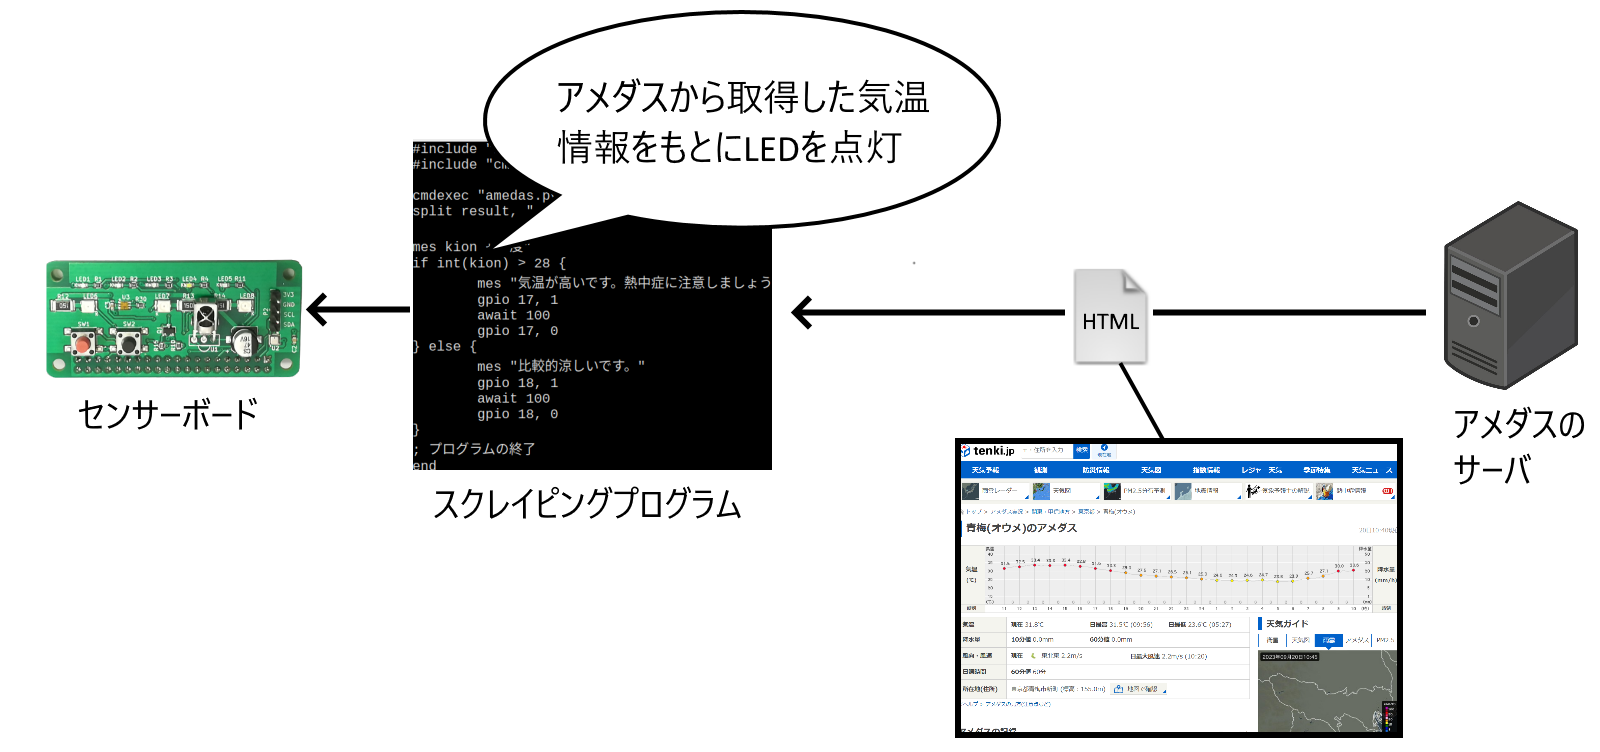
\includegraphics[width=\textwidth]{slide08-img006.png}
    \end{figure}
\end{frame}

\begin{frame}[fragile]
	\frametitle{\large{スクレイピングで得た情報をつかってみよう:テキスト P.\pageref{1:P:scraping}-}~~~\raisebox{-3mm}{
\includegraphics[width=0.1\textwidth]{raspberry}}}
    \begin{itemize}
        \item ブラウザで右クリックをして、「検証」を選択すると、開いているページとHTMLの対応を見ることができます。
        \item ほしい情報がHTMLのどこにあるのかを探してみましょう。
    \end{itemize}
    \begin{figure}
      \centering
      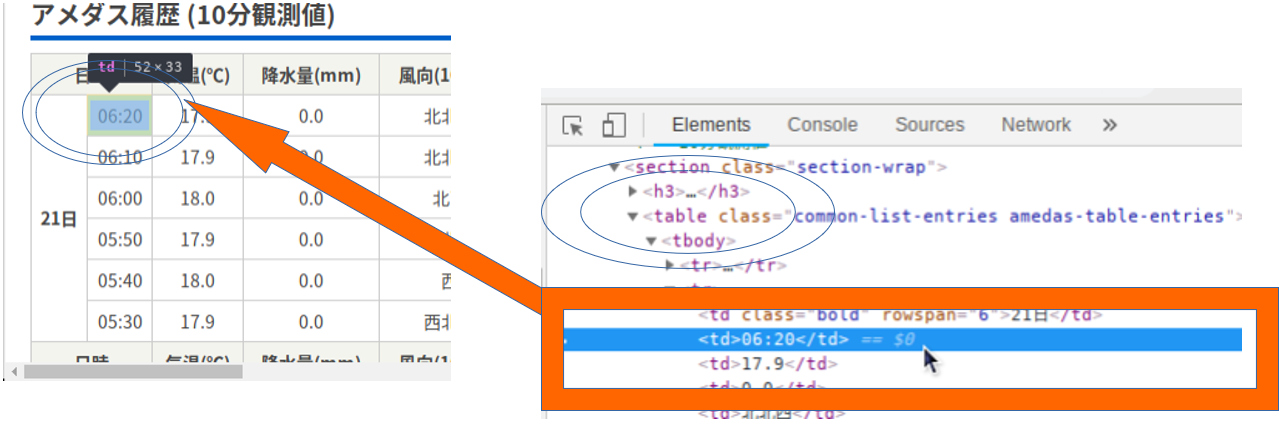
\includegraphics[width=\textwidth]{slide08-img008.png}
    \end{figure}
\end{frame}

\begin{frame}[fragile]
	\frametitle{\large{スクレイピングで得た情報をつかってみよう:テキスト P.\pageref{1:P:scraping}-}~~~\raisebox{-3mm}{
\includegraphics[width=0.1\textwidth]{raspberry}}}
      \textbf{教科書をよみながら、例題をやってみよう}
				\begin{itemize}
					\item \ref*{1:E:amedas}
					\item \ref*{1:E:amedasLess}
					\item \ref*{1:E:amedasSensor}
				\end{itemize}
      \vfill
      \textbf{速く終わった子は、次の問題をやってみよう}
				\begin{itemize}
					\item \ref*{1:Q:amedas1}, \ref*{1:Q:amedas2}, \ref*{1:Q:amedas3}, \ref*{1:Q:amedas4}
					\item \ref*{1:Q:amedas5}, \ref*{1:Q:amedas6}, \ref*{1:Q:amedas7}, \ref*{1:Q:amedas8}
				\end{itemize}
      \vfill
      \textbf{わからないことは、放っておかず、すぐに TA に聞きましょう}
\end{frame}

\begin{frame}[fragile]
	\frametitle{\large{スクレイピングで得た情報をつかってみよう:テキスト P.\pageref{1:P:scraping}-}~~~\raisebox{-3mm}{
\includegraphics[width=0.1\textwidth]{raspberry}}}
    \begin{itemize}
        \item いろんなWebサイトをスクレイピングしてみましょう。
        \item 得た情報を使って何ができるか、考えてみましょう。
    \end{itemize}
    \begin{figure}
      \centering
      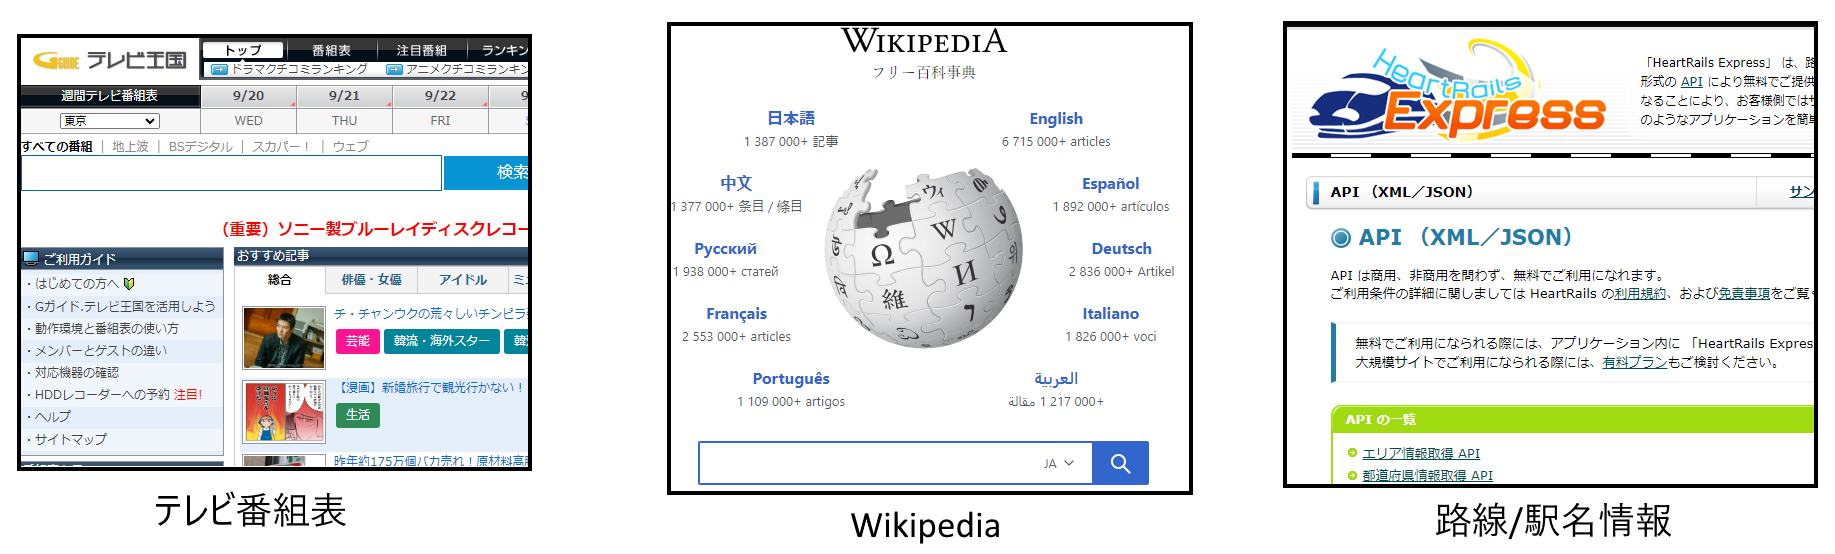
\includegraphics[width=\textwidth]{slide08-img007.png}
    \end{figure}
\end{frame}

\begin{frame}[fragile]
	\frametitle{\large{スクレイピングで得た情報をつかってみよう:テキスト P.\pageref{1:P:scraping}-}~~~\raisebox{-3mm}{
\includegraphics[width=0.1\textwidth]{raspberry}}}
      \textbf{教科書をよみながら、例題をやってみよう}
				\begin{itemize}
					\item \ref*{1:E:TV}
					\item \ref*{1:E:Weblio}
					\item \ref*{1:E:station}
					\item \ref*{1:E:postNum}
					\item \ref*{1:E:wikipedia}
				\end{itemize}
      \vfill
      \textbf{速く終わった子は、次の問題をやってみよう}
				\begin{itemize}
					\item \ref*{1:Q:TV}, \ref*{1:Q:weblio}, \ref*{1:Q:station}
					\item \ref*{1:Q:postNum}, \ref*{1:Q:wikipedia}
				\end{itemize}
      \vfill
      \textbf{わからないことは、放っておかず、すぐに TA に聞きましょう}
\end{frame}

